\documentclass[margin=0.5cm]{standalone}

\usepackage{tikz}
\usepackage{newtxtext}
\usepackage{newtxmath}
\usepackage{xcolor}

\definecolor{starfishyellow}{HTML}{FFBD59}

\begin{document}

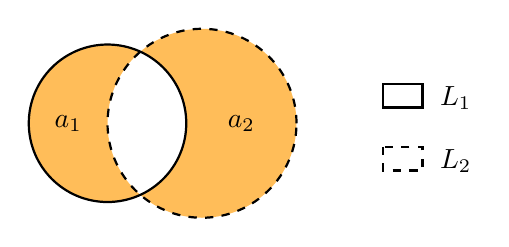
\begin{tikzpicture}
\fill[even odd rule, starfishyellow] (0,0) circle (1cm) (1.2,0) circle (1.2cm);
\draw[thick] (0,0) circle (1cm);
\draw[dashed, thick] (1.2,0) circle (1.2cm);
\node at (-0.5,0) {$a_1$};
\node at (1.7,0) {$a_2$};

\draw[thick] (3.5,0.5) rectangle ++(0.5,-0.3);
\draw[dashed, thick] (3.5,-0.3) rectangle ++(0.5,-0.3);
\node[anchor=west] at (4.1, 0.32) {$L_1$};
\node[anchor=west] at (4.1, -0.48) {$L_2$};
\end{tikzpicture}

\end{document}
